\subsection{Group Methods}
\label{sec:methods.structured.group}

% Author: Flo
  
Since it is often useful to select or discard a group of features at once,
features can be grouped into feature-groups. Weights can now be assigned to
whole groups by minimization techniques and groups with weights close to $0$ can be
eliminated. An algorithm that uses this approach is the Group Lasso. 

This approach does not necessarily exclude the possibility to select single
features inside feature groups as well. As a matter of fact some methods
(e.g. the Sparse Group Lasso Regularization) perform feature-group selection and
feature selection at once (\cite{Tang:04}).

\begin{figure}[!ht]
  \centering 
  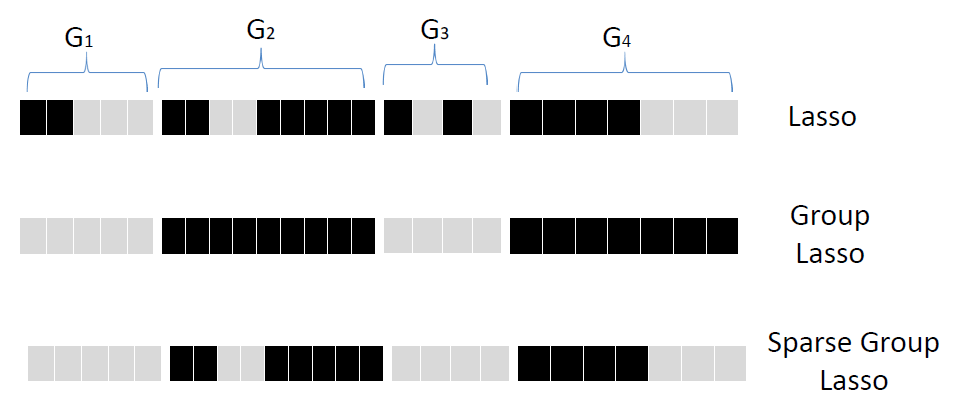
\includegraphics[width=0.8\textwidth]{chapters/methods/structured/group_lasso}
  \caption{Reprinted from (\cite{Tang:04}). Illustration of Lasso, Group Lasso
  and Sparse Group Lasso.
  Features can be grouped into 4 disjoint groups {G1,G2,G3,G4}. Each cell denotes a feature and light color
represents the corresponding cell with coefficient zero (\cite{Tang:04}).}
  \label{fig:methods.structured.group.lasso}
\end{figure}

In Figure \ref{fig:methods.structured.group.lasso} you can see some examples of
how Lasso, Group Lasso and Sparse Group Lasso can select features. 

Sometimes the given data structure might suggest overlapping feature-groups,
where a feature can belong to more than one group. This case is no longer
handled correctly by the Sparse Group Lasso-method. Some methods that handle
this scenario are:

\begin{itemize}
  \item \cite{Liu:10}
  \item \cite{Kim:10}
  \item \cite{Jenatton:10}
  \item \cite{Jacob:09}
\end{itemize}

% TODO: Concrete methods





